\subsection{Peak Traffic Demand}\label{subsec:peakratio}

The Sandvine Reports show that although the mean traffic demand has remained
stable for the past few years, demand during prime-time hours has increased
drastically~\cite{sandvine20141h}. Although, these reports present a good view 
into aggregate usage 
patterns over a month, they neglect to analyze usage characteristics 
individually. 
We measure the disparity between the daily 95 percentile of the peak and 
mean usage of each household, and call this the \emph{Peak-Ratio}.

\begin{figure}[t]
\begin{minipage}{1\linewidth}
\centering
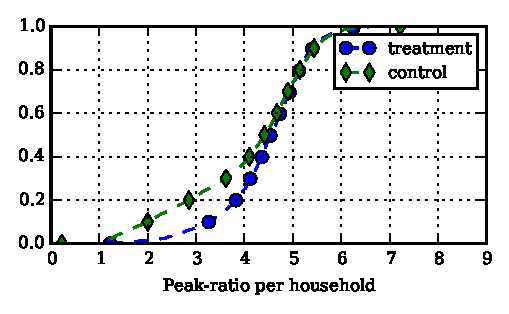
\includegraphics[width=1\linewidth]{figures/peakratio-CDF-devices-MEAN.pdf}
\caption{Distribution of peak ratio for subscribers in the treatment and 
control groups.}
\label{fig:CDF-peak-ratio-mean}
\end{minipage}
\end{figure}

Figure ~\ref{fig:CDF-peak-ratio-mean} plots the mean peak-ratio for each 
device in the \treatment{} and \control{} sets.
For 60 percent of the users with the most disparity between their
95 percentile and mean demand in a day, the peak-ratio is unaffected by
service upgrade. For 40 percent of the users with a low peak ratio in the 
control
group, users in the \treatment{} group have a higher peak ratio.
Following our observations of a lower prime-time ratio of the  
\treatment{} set (section~\ref{subsec:primetime}), this implies that there are 
households in the \test set that achieve a peak-ratio $>$ 1, but not during the 
prime-time hour. We believe that these households might actually be small 
businesses or work-at-home users that peak during daytime hours instead of 
evening hours.